% This is "sig-alternate.tex" V2.0 May 2012
% This file should be compiled with V2.5 of "sig-alternate.cls" May 2012
%
% This example file demonstrates the use of the 'sig-alternate.cls'
% V2.5 LaTeX2e document class file. It is for those submitting
% articles to ACM Conference Proceedings WHO DO NOT WISH TO
% STRICTLY ADHERE TO THE SIGS (PUBS-BOARD-ENDORSED) STYLE.
% The 'sig-alternate.cls' file will produce a similar-looking,
% albeit, 'tighter' paper resulting in, invariably, fewer pages.
%
% ----------------------------------------------------------------------------------------------------------------
% This .tex file (and associated .cls V2.5) produces:
%       1) The Permission Statement
%       2) The Conference (location) Info information
%       3) The Copyright Line with ACM data
%       4) NO page numbers
%
% as against the acm_proc_article-sp.cls file which
% DOES NOT produce 1) thru' 3) above.
%
% Using 'sig-alternate.cls' you have control, however, from within
% the source .tex file, over both the CopyrightYear
% (defaulted to 200X) and the ACM Copyright Data
% (defaulted to X-XXXXX-XX-X/XX/XX).
% e.g.
% \CopyrightYear{2007} will cause 2007 to appear in the copyright line.
% \crdata{0-12345-67-8/90/12} will cause 0-12345-67-8/90/12 to appear in the copyright line.
%
% ---------------------------------------------------------------------------------------------------------------
% This .tex source is an example which *does* use
% the .bib file (from which the .bbl file % is produced).
% REMEMBER HOWEVER: After having produced the .bbl file,
% and prior to final submission, you *NEED* to 'insert'
% your .bbl file into your source .tex file so as to provide
% ONE 'self-contained' source file.
%
% ================= IF YOU HAVE QUESTIONS =======================
% Questions regarding the SIGS styles, SIGS policies and
% procedures, Conferences etc. should be sent to
% Adrienne Griscti (griscti@acm.org)
%
% Technical questions _only_ to
% Gerald Murray (murray@hq.acm.org)
% ===============================================================
%
% For tracking purposes - this is V2.0 - May 2012

\documentclass{sig-alternate}
% *** CITATION PACKAGES ***
%
\usepackage{cite}
% cite.sty was written by Donald Arseneau
% V1.6 and later of IEEEtran pre-defines the format of the cite.sty package
% \cite{} output to follow that of IEEE. Loading the cite package will
% result in citation numbers being automatically sorted and properly
% "compressed/ranged". e.g., [1], [9], [2], [7], [5], [6] without using
% cite.sty will become [1], [2], [5]--[7], [9] using cite.sty. cite.sty's
% \cite will automatically add leading space, if needed. Use cite.sty's
% noadjust option (cite.sty V3.8 and later) if you want to turn this off.
% cite.sty is already installed on most LaTeX systems. Be sure and use
% version 4.0 (2003-05-27) and later if using hyperref.sty. cite.sty does
% not currently provide for hyperlinked citations.
% The latest version can be obtained at:
% http://www.ctan.org/tex-archive/macros/latex/contrib/cite/
% The documentation is contained in the cite.sty file itself.






% *** GRAPHICS RELATED PACKAGES ***
%
%\if CLASSINFOpdf
  \usepackage{graphicx}
  \usepackage{epstopdf}
 % \usepackage{auto-pst-pdf}
  % declare the path(s) where your graphic files are
  % \graphicspath{{./eps}{./pdf/}{./jpeg/}}
  % and their extensions so you won't have to specify these with
  % every instance of \includegraphics
  \DeclareGraphicsExtensions{.eps,.pdf,.jpeg,.png,.ps}
%\else
  % or other class option (dvipsone, dvipdf, if not using dvips). graphicx
  % will default to the driver specified in the system graphics.cfg if no
  % driver is specified.
 % \usepackage[dvips]{graphicx}
  % declare the path(s) where your graphic files are
  % \graphicspath{{./eps/}}
  % and their extensions so you won't have to specify these with
  % every instance of \includegraphics
 % \DeclareGraphicsExtensions{.eps}
%\fi
% graphicx was written by David Carlisle and Sebastian Rahtz. It is
% required if you want graphics, photos, etc. graphicx.sty is already
% installed on most LaTeX systems. The latest version and documentation can
% be obtained at: 
% http://www.ctan.org/tex-archive/macros/latex/required/graphics/
% Another good source of documentation is "Using Imported Graphics in
% LaTeX2e" by Keith Reckdahl which can be found as epslatex.ps or
% epslatex.pdf at: http://www.ctan.org/tex-archive/info/
%
% latex, and pdflatex in dvi mode, support graphics in encapsulated
% postscript (.eps) format. pdflatex in pdf mode supports graphics
% in .pdf, .jpeg, .png and .mps (metapost) formats. Users should ensure
% that all non-photo figures use a vector format (.eps, .pdf, .mps) and
% not a bitmapped formats (.jpeg, .png). IEEE frowns on bitmapped formats
% which can result in "jaggedy"/blurry rendering of lines and letters as
% well as large increases in file sizes.
%
% You can find documentation about the pdfTeX application at:
% http://www.tug.org/applications/pdftex

% *** ALIGNMENT PACKAGES ***
%
%\usepackage{array}
% Frank Mittelbach's and David Carlisle's array.sty patches and improves
% the standard LaTeX2e array and tabular environments to provide better
% appearance and additional user controls. As the default LaTeX2e table
% generation code is lacking to the point of almost being broken with
% respect to the quality of the end results, all users are strongly
% advised to use an enhanced (at the very least that provided by array.sty)
% set of table tools. array.sty is already installed on most systems. The
% latest version and documentation can be obtained at:
% http://www.ctan.org/tex-archive/macros/latex/required/tools/
\usepackage{balance}
\usepackage{mdframed}
\usepackage{enumitem}
%\usepackage{mdwmath}
%\usepackage{mdwtab}
% Also highly recommended is Mark Wooding's extremely powerful MDW tools,
% especially mdwmath.sty and mdwtab.sty which are used to format equations
% and tables, respectively. The MDWtools set is already installed on most
% LaTeX systems. The lastest version and documentation is available at:
% http://www.ctan.org/tex-archive/macros/latex/contrib/mdwtools

\begin{document}
%
% --- Author Metadata here ---
\conferenceinfo{International Conference on Software Engineering}{2014 Hyderbad, India}
%\CopyrightYear{2007} % Allows default copyright year (20XX) to be over-ridden - IF NEED BE.
%\crdata{0-12345-67-8/90/01}  % Allows default copyright data (0-89791-88-6/97/05) to be over-ridden - IF NEED BE.
% --- End of Author Metadata ---

\title{Experiences Gamifying Developer Adoption\\ of Practices and Tools}
% 
% You need the command \numberofauthors to handle the 'placement
% and alignment' of the authors beneath the title.
%
% For aesthetic reasons, we recommend 'three authors at a time'
% i.e. three 'name/affiliation blocks' be placed beneath the title.
%
% NOTE: You are NOT restricted in how many 'rows' of
% "name/affiliations" may appear. We just ask that you restrict
% the number of 'columns' to three.
%
% Because of the available 'opening page real-estate'
% we ask you to refrain from putting more than six authors
% (two rows with three columns) beneath the article title.
% More than six makes the first-page appear very cluttered indeed.
%
% Use the \alignauthor commands to handle the names
% and affiliations for an 'aesthetic maximum' of six authors.
% Add names, affiliations, addresses for
% the seventh etc. author(s) as the argument for the
% \additionalauthors command.
% These 'additional authors' will be output/set for you
% without further effort on your part as the last section in
% the body of your article BEFORE References or any Appendices.

\numberofauthors{3} %  in this sample file, there are a *total*
% of EIGHT authors. SIX appear on the 'first-page' (for formatting
% reasons) and the remaining two appear in the \additionalauthors section.
%
% author names and affiliations
% use a multiple column layout for up to three different
% affiliations
\author{
\alignauthor
Will Snipes\\
\affaddr{ABB Corporate Research}\\
\affaddr{Industrial Software Systems}\\
\affaddr{Raleigh, NC USA}\\
\email{will.snipes@us.abb.com}
\and
\alignauthor
Anil R. Nair\\
\affaddr{ABB Corporate Research}\\
\affaddr{Industrial Software Systems}\\
\affaddr{Bangalore, India}\\
\email{anil.nair@in.abb.com}
\and
\alignauthor
Emerson Murphy-Hill\\
\affaddr{NC State University}\\
\affaddr{Computer Science}\\
\affaddr{Raleigh, N.C. USA}\\
\email{emerson@csc.ncsu.edu}\\
}



\maketitle
\begin{abstract}

As software development practices evolve, toolsmiths face the continuous challenge of getting developers to adopt new practices and tools.   We tested an idea with industrial software developers that adding game-like feedback to the development environment would improve adoption of tools and practices for code navigation.  We present results from a pre-study survey of 130 developers' opinions on gamification and motivation, usage data from a pilot with an intact team of six developers of a game on code navigation practices, and feedback collected in post-pilot interviews.  Our pre-study survey showed that most developers were interested in gamification, though some have strong negative opinions.  Pilot results show that two of the six pilot developers adjusted their practices when presented with competitive game elements.
%We found that a software engineering game with competitive elements influences some developers towards changing their practices.
%We also learned that demonstrating significant improvement can be difficult and that developers want more proactive messages and recommendations on ways they can improve.
%
% In addition to training, discussing, and presenting software engineering practices and tools, we demonstrate a method to both motivate and monitor their adoption through a tool embedded in the Integrated Development Environment (IDE).  
%
%We determine through a survey of 130 developers the things we can do to motivate them to adopt 
%Blaze monitors developer practice and tool use over the long term and reports the lasting change a tool deployment or communication effort makes in everyday habits. 
%
% Embedding Blaze in the developer's work environment as a Visual Studio extension captures developer work patterns while giving feedback to users on their practices.   Blaze encourages everyone to use the new practices by assigning points to specific commands and tools.  
% With a rich data source, we evaluate developer practices, define metrics that give individual feedback, and create an environment for developers to see how they are doing compared with their teammates.  
%
%Data collected from the pilot group show a dichotomy of navigation and code understanding practices used by developers even the same developer in different situations.  We observed that the duration of an edit session is more correlated with categories of activity that benefit from improved practices and tools. The Blaze tool was well received by most participants, however, navigation practices were not significantly affected by the Blaze feedback mechanism.  We conclude that more proactive interventions are necessary to encourage developers to change their code navigation habits.
\end{abstract}

\category{D.2.9}{Software}{Software Engineering} {Management} [Productivity]

\terms{Management, Economics, Human computer interaction}

\keywords{Development, Productivity, Code Navigation}

\section{Introduction}

Sascha is a developer with years of experience maintaining code, who knows how to navigate through code fairly well.  Sascha heard about some other navigation tools, but kept using the built-in features of the Visual Studio IDE mainly out of habit.  When Sascha's company started a game around code navigation in Visual Studio, he became interested in being a part of the fun.  Sascha tried the code navigation tools and practices that were part of the game and soon found himself at the top of the game's leaderboard.  After learning the new practices Sascha spends less time navigating code to accomplish his maintenance tasks.

Like Sascha, software developers who maintain code face challenges of navigating an existing code base to incorporate changes as they build new features or fix bugs.  Toolsmiths respond to these challenges by creating new tools for assisting developers through difficult activities like code navigation.  However, as new practices and tools become available, developers may be motivated to start using them unless they interact with a peer developer who promotes them\cite{wbsnipes:Hill2011Peer}.    Of course they are intrinsically motivated to improve, but urgent demands interfere with experimenting using new tools and they become less efficient than otherwise possible.  Thus, we need to both communicate with and motivate developers like Sascha to start using new tools.  

One option for motivating people to adopt new practices is to apply elements of game mechanics or ``gamify'' the practice. Gamification is the incorporation of game elements into an activity that people do not typically consider a game\cite{2013Oxford}.  We envisioned a tool in our prior work that would motivate developers by providing constant feedback and allowing them to compare their improvements to how their peers are doing  \cite{Snipes2013Towards}.  This tool, called Blaze, creates a competitive game with continuous feedback on how well the developer adopts the improved practice.  The more they change their practices to adopt new techniques or tools, the higher they score in the game. 

Would software developers writing serious software be motivated by this gamification concept? To answer this question, this work contributes an assessment of developers' response to game-like elements tied to their use of new tools and practices.  We assess 130 developers' response and relevant concerns about the idea of gamification through a web-based survey.  We piloted Blaze, our tool that introduces game elements focused on improving navigation practices into the developer's IDE.  Developers' reactions to gamification were mostly positive with a few detractors, and results of piloting show that game elements influence some developers, but have no effect on others' use of tools and practices.

The rest of this paper is organized as follows:  Section 2 reviews related work, Section 3 reviews results from the pre-study survey, Section 4 discusses the design considerations for developing the Blaze tool/game, Section 5 discusses the design of the Blaze pilot study,  Section 6 results from the pilot study and post-pilot survey, Section 7 covers threats to validity, and Section 8 has our conclusions.

\section{Related Work}

The two areas of related work we discuss are research studies using other monitoring methods and studies applying gamification to other areas.

\subsection{Monitoring Practice Studies }

Robillard, Coelho and Murphy explore hypotheses around how developers can be more effective at performing a maintenance task \cite{wbsnipes:Robillard2004How}.  Robillard et al. say developers are more successful finding and fixing bugs when they create a detailed plan for implementing a change, use structured navigation with keyword search or cross-reference search, and only review methods once during their search.  We build on their work by testing methods for increasing the use of structured navigation in developers' everyday practice.

Johnson and Kou defined Zorro\cite{V:Johnson2007Automated}, a system for detecting whether developers use Test Driven Development techniques based on data from Hackystat.  Zorro divides development activities into episodes delimited by events such as configuration management code check-in, start of a unit test run, or start of a build.  Using the distinct events developers follow within these episodes, Zorro determines whether the episode followed Test-Driven Development practices per their classic definition of test first - code - test pass, or a different scenario.  In two student-based studies comparing Zorro classifications with a simultaneous observational screen video, Zorro achieved between 70\% \cite{Kou2010Operational} and 89\% \cite{V:Johnson2007Automated} accuracy when classifying episodes into their proper TDD scenarios.  The studies did not, however, attempt to use or evaluate the influence of instant feedback aimed at encouraging participants to follow the classic definition of Test Driven Development.  In our study, we attempt to present data collected directly to developers in order to influence them to change their practices.

Murphy-Hill, Parnin, and Black \cite{V:MurphyHill2012How} use the Mylyn Monitor to explore whether or not developers use the automated refactoring tools present in Eclipse.  They look for specific refactoring commands in Eclipse and determine the amount of time developers use tools versus hand refactoring the code.  For this study, we focus on code navigation as a high-value area for improving developer efficiency.

The Pro Metrics (PROM) tool provides a framework for collecting data for further analysis from tools used by developers.\cite{Coman2009Casestudy}  It provides a flexible data model and a plug-in architecture to facilitate collection from different data sources.  Studies conducted using PROM include a series of studies on trends in time spent Pair Programming \cite{Coman2008Investigating}, benefits of refactoring on productivity \cite{Moser2008Case}, impact of refactoring on re-usability \cite{Moser2006Does}, and prediction of effort \cite{Abrahamsson2007Effort}.  Studies using the PROM tool correlate the time spent editing with code metrics obtained through source code analysis.  Applying these data to specific research questions ,such as whether refactoring improves productivity \cite{Moser2008Case}, shows the utility of combining automated effort data with code metric data.  Taking a different focus on techniques, our study used more detailed events captured from the IDE  to detect commands the uses to navigating through the code in addition to knowing duration of edit sessions for code modules.

Murphy-Hill et al. study a large usage history data set and apply several different algorithms to accurately suggest IDE commands to novice users\cite{MurphyHill2012Improving}.  Algorithms based on command history performed well particularly when synchronized chronologically with the recipient's usage history. Novice users were better served by recommendation algorithms that did not require a long history, while more expert users benefited from more sophisticated algorithms that included more history. The ``Most Widely Used'' algorithm recommends commands based on the collective usage profile of the team and performed nearly as well as the more sophisticated algorithms. The paper presents the methodology for making recommendations and evaluating their accuracy. Our work takes a further step evaluating how well tools can influence developers to use a specific recommended commands.

\subsection{Gamification}

When discussing gamification, folks raise a concern about replacing an activity like software development, which is intrinsically motivated, with extrinsic motivation provided by points and achievements.  To discover what is behind this concern, we reviewed several studies on motivation and gamification. 

Beecham and colleagues provide a thorough analysis of existing literature on studies of motivation in Software Engineering \cite{Beecham2008Motivation}.  They claim that the most common motivator found in cited references is ''the work''. The list of de-motivators is also useful with common job satisfaction items like stress and inequity in recognition, plus poor quality software (low accomplishment) and lack of influence in decision making. The paper also lists characteristics of people in the professions including need for independence (autonomy), desire to learn new skills and tackle new challenges. 

Maehr proposes an affirmative theory whereby  individuals achieve as a member of a social group, choosing the behavior that meets the expectations and values of the group that is significant to them\cite{wbsnipes:MaehrCulture}.  A key factor in raising achievement motivation is establishing a social group where the person is motivated to belong and excel.  Maehr states that since achievement behaviors can be triggered by circumstance, they are present in most people regardless of background. 

Hamari et al. analyze achievements patterns in game systems and provide guidance on defining successful achievement systems.  They recommend  achievement awards be setup as a secondary form of scoring so players have multiple objectives available for a particular game.  Players should feel like they earned achievements in the game; they should not be given for trivial tasks.

Singer and Schneider demonstrate the use of a message board and points for encouraging students to increase their frequency of commits to the source code repository \cite{Singer2012It}.  The communication mechanism enabled students to see each others' progress and resulted in more frequent commits than baseline.  Participants valued the communication and collaboration aspect and some valued the competition enough to change their opinion on optimum commit frequency.  The subsequent thesis by Singer \cite{Singer2013a} describes results of an experiment conducted across two iterations of a class where active feedback on commits was deployed to one course and another course served as the control group where commit frequency was simply monitored.  Results show an increase in the frequency of commits at a statistically significant level.  This study uses fine grained instrumentation to identify practices used between commits such as structured navigation.

Dubois and Tamburrelli discuss theoretical concepts behind applying gamification to software development \cite{Dubois2013Understanding}. Their approach is to consider how gamification could be applied throughout the software development life-cycle to motivate many practices in different phases.  They provide guidance on assessing gamification in the software development domain including analyzing the actors and game mechanics, defining integration with existing tools and processes, and designing the evaluation of results.  Dubois and Tamburrelli demonstrate this guidance using a study of students working on a class project.  Defining a control group and subject group of students, both groups receive the same feedback about their code comments, test coverage, code size, and static analysis rule violations.  The subject group can see each others' rankings while the control group only sees their personal rankings.  Results, though inconclusive, show competition increases the desired results.  In our study, we provide participants with both individual feedback and anonymized competitive feedback and seek to observe a change in their behavior.

\section{Pre-study Survey}

\subsection{Pre-study Background}

Understanding the concerns with maintaining developers'  intrinsic motivation while adding elements of achievement motivation, we conducted an assessment survey questionnaire to determine whether the ABB developer community would be receptive to a gamification approach to software development.  The developer survey received over 130 responses from software developers at ABB.

\subsection{Pre-study Survey Results}

Using a question from the Saatchi and Saatchi survey \cite{wbsnipes:SaatchiGameification} as directly as possible, we asked developers at ABB ``How interested they would be in working for a company that incorporated some aspects of games into software engineering tools as a way to increase productivity in the workplace''?  We segmented results by country in Figure \ref{fig:gamification} and found gamification of software engineering is more interesting to developers in India, Poland, and Finland than in other major countries.  The responses indicate 75-88\% of developers in India, Poland, and Finland were at least somewhat interested.  For the US, Sweden, and Switzerland the responses indicate 60-65\% are at least somewhat interested.  

Comments from participants reflected a more interesting controversial reaction than these measurements might otherwise indicate.  A developer from India said ``Gamification is a juvenile way of getting programmers to do something that you want.''  A different respondent expressed a concern that ``Gamification of best practices can have nasty side effects.''  Another participant said ``there is already high a level of competition between software development teams..'' indicating they are under considerable pressured to get the work done.  Another developer reacted with a statement that identifies the kind of intrinsic motivation we hope for ``I am using practices and tools because I want to do my job well',' indicating that gamification was unnecessary to motivate people to improve.

On the positive side, a developer from Poland said, ``In a previous work place we had a 'game' between developers - scoring broken/unbroken builds and new/passed/failed tests. It was helping to improve quality and it worked well. [It is] recommended especially for junior developers. ''  Other comments indicated competition or points are acceptable ``as long as it doesn't interrupt or slow down my work. ''

Because we nearly identically reused their original question, we compare the overall response from our survey to the Saatchi and Saatchi survey\cite{wbsnipes:SaatchiGameification} upon which this question was based.  Our results land on both sides of the 75\% mark reported by the Saatchi and Saatchi study.  

\begin{figure}
	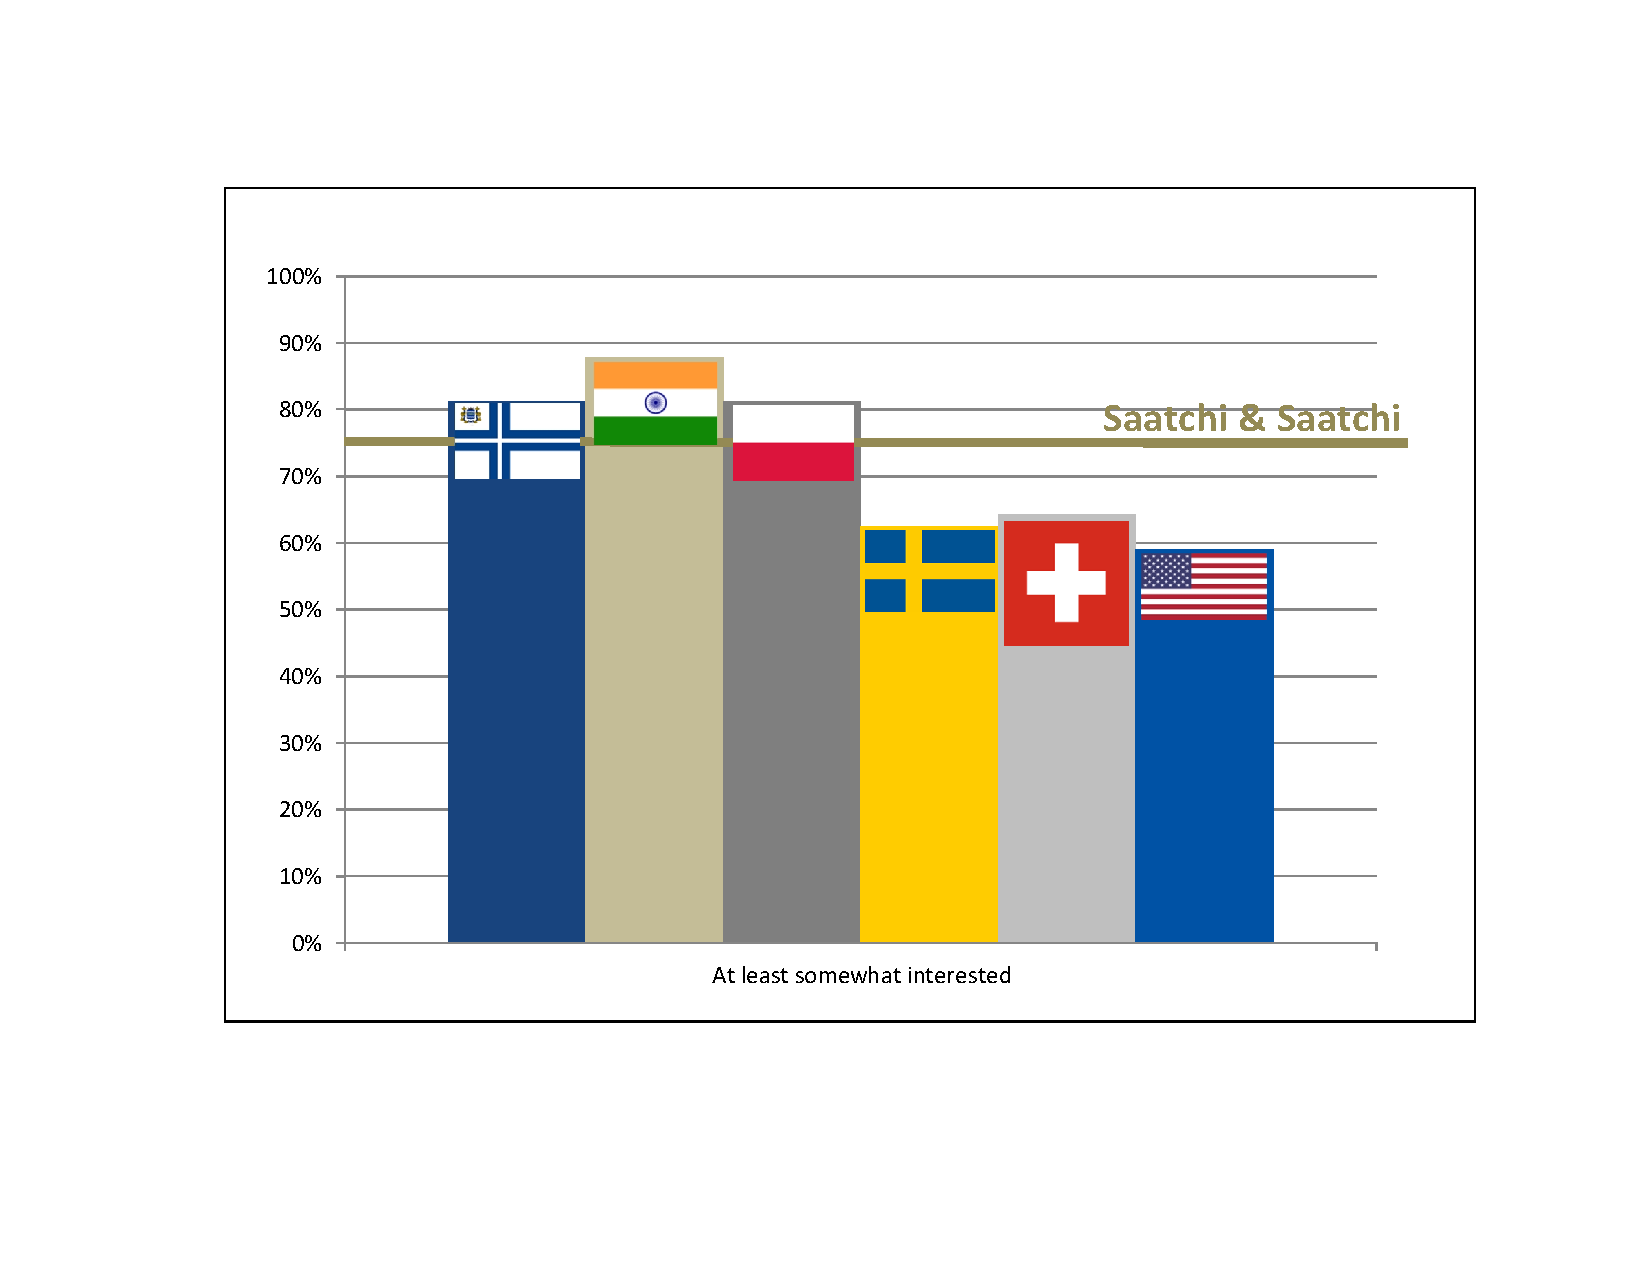
\includegraphics[width=3.4in]{gamificationquestion.pdf}
	\caption{Acceptance of gamification}
	\label{fig:gamification}
\end{figure}

We asked developers how likely they would be to try tools and practices recommended to them through an automated usage tracking system.  Answers showed 95\% of the developers surveyed are likely to try the recommended tools and practices.  Thus, a recommendation system would positively impact the deployment of software engineering tools and practices at ABB.

Another question was whether sharing detailed usage information with colleagues and the company as a whole would be a concern for developers.  The question provided a graduated scale for the scope of who data was shared with and divided the questions between whether sharing was anonymous or not. Figure \ref{fig:comfortwithsharing}  shows over 90\% of respondents are comfortable with sharing either anonymous or non-anonymous information with their team members. 
Their comfort level decreases as the scope of who the information is shared with increases.  People were less comfortable sharing with anyone (the category for people outside ABB) particularly if the data was not kept anonymous.  
The first conclusion from these questions on sharing data is that people are very willing to share information that could help their team. Second, sharing within the company is acceptable if we take care to make the data anonymous.

\begin{figure}
	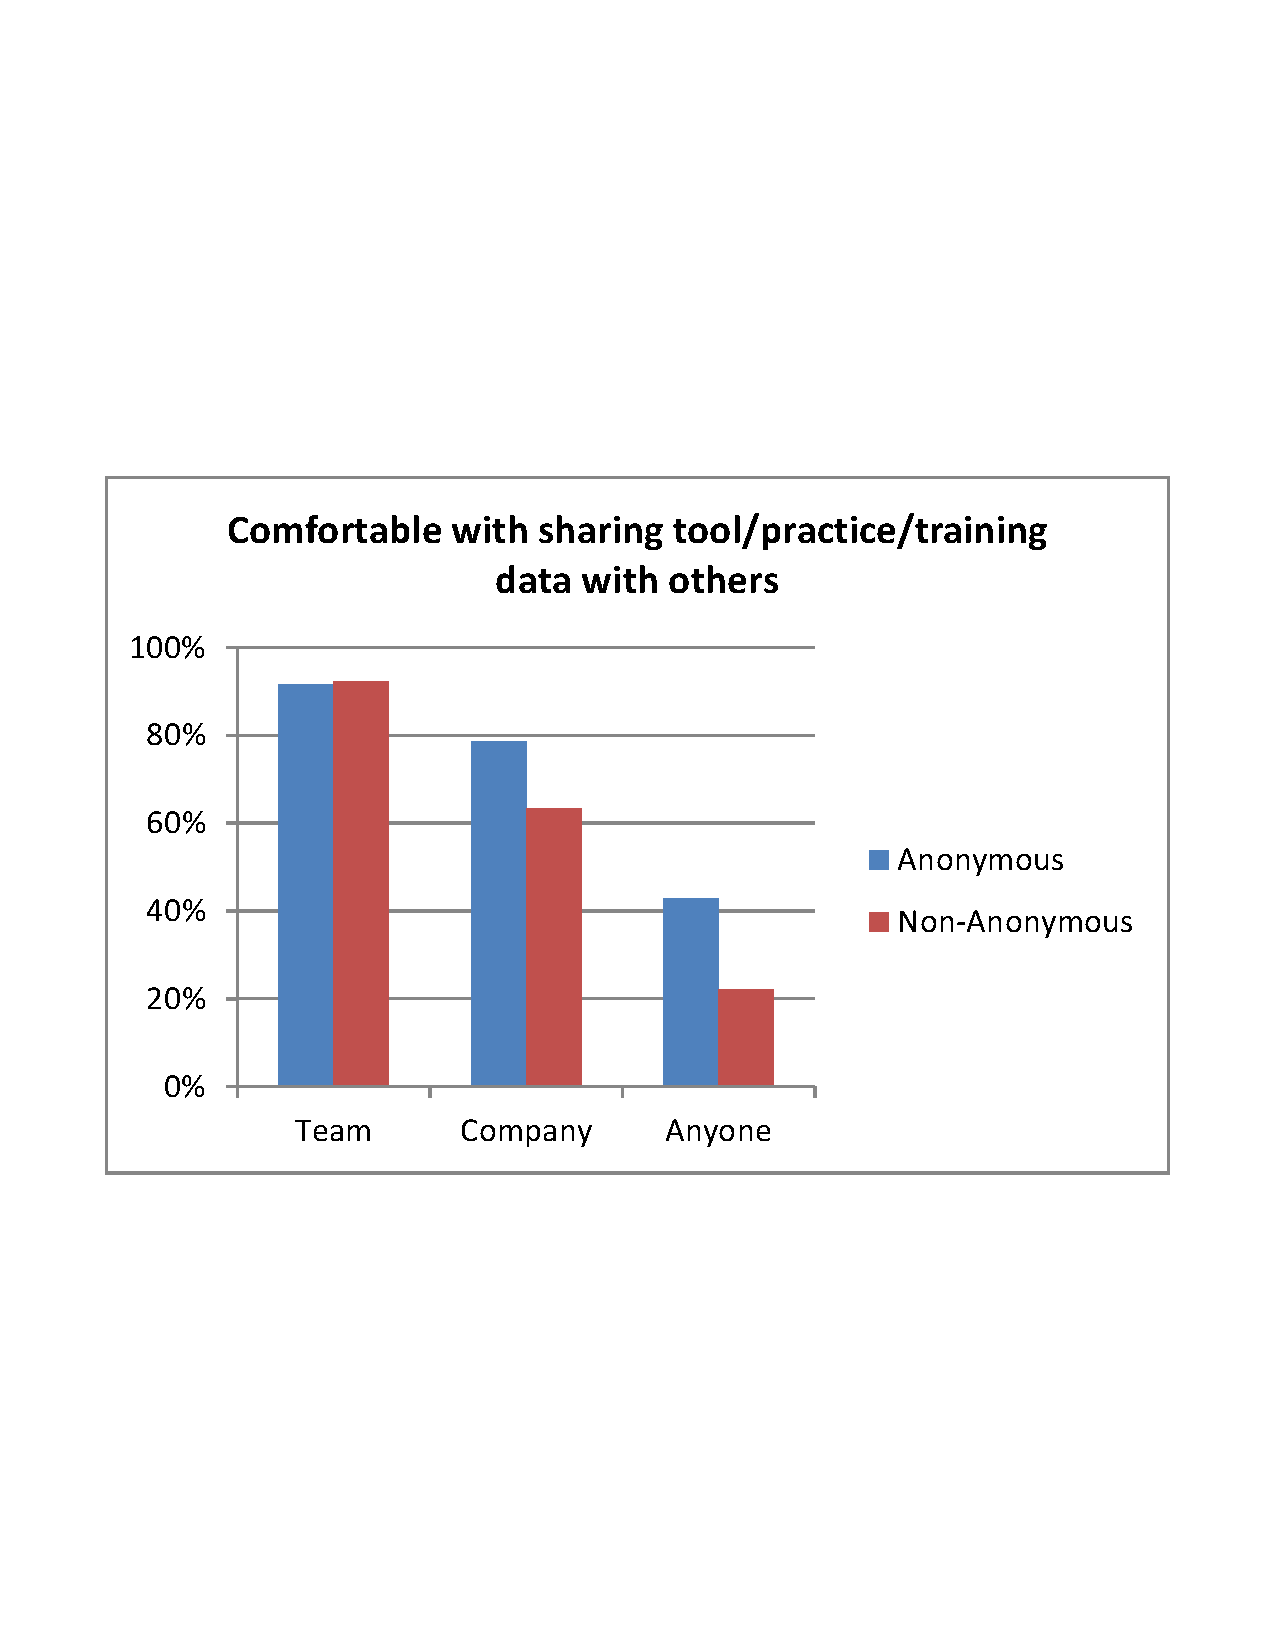
\includegraphics[width=3.4in]{ComfortWithSharing.pdf}
	\caption{Comfort with sharing usage information}
	\label{fig:comfortwithsharing}
\end{figure}

We asked developers what would motivate them to use tools and practices and gave them four choices to rank.  In Figure \ref{fig:toolandpracticemotivators}, we see that 75\% of respondents ranked coworker recommendation in 1st or 2nd place.  Of several comments, a developer in Sweden captured the following scene, ``[The] most motivating [thing] is when a new practice / tool is discussed during a continuous improvement meeting or even coffee break, where one co-developer tells about the benefits and there is a joint discussion on where it (tool or practice) could be best applied.''  

The team goal ranked second behind coworker recommendation.  This response indicated that developers would be motivated to use new tools and practices if that helped their team in a competion between development teams at ABB.  The result shows that team competition would be first or second on the list for  47\% of developers to motivate their use of practices or tools.  

Just behind team competition is management mandate where developers would be asked to follow specific practices by the organization.  The lowest was having badges posted on their social network profile where 32\% ranked this in 1st or 2nd place.   Badges and management mandate received the most negative written comments in the survey.  A developer from the United States captured the lower opinion of badges that several participants expressed ``I am motivated because ABB allows me to choose the tools that best work for me. A badge will not really do anything for me.''  We conclude that a facility to share coworker recommendations on tools and practices has the best opportunity to increase their adoption.  
 
\begin{figure}
	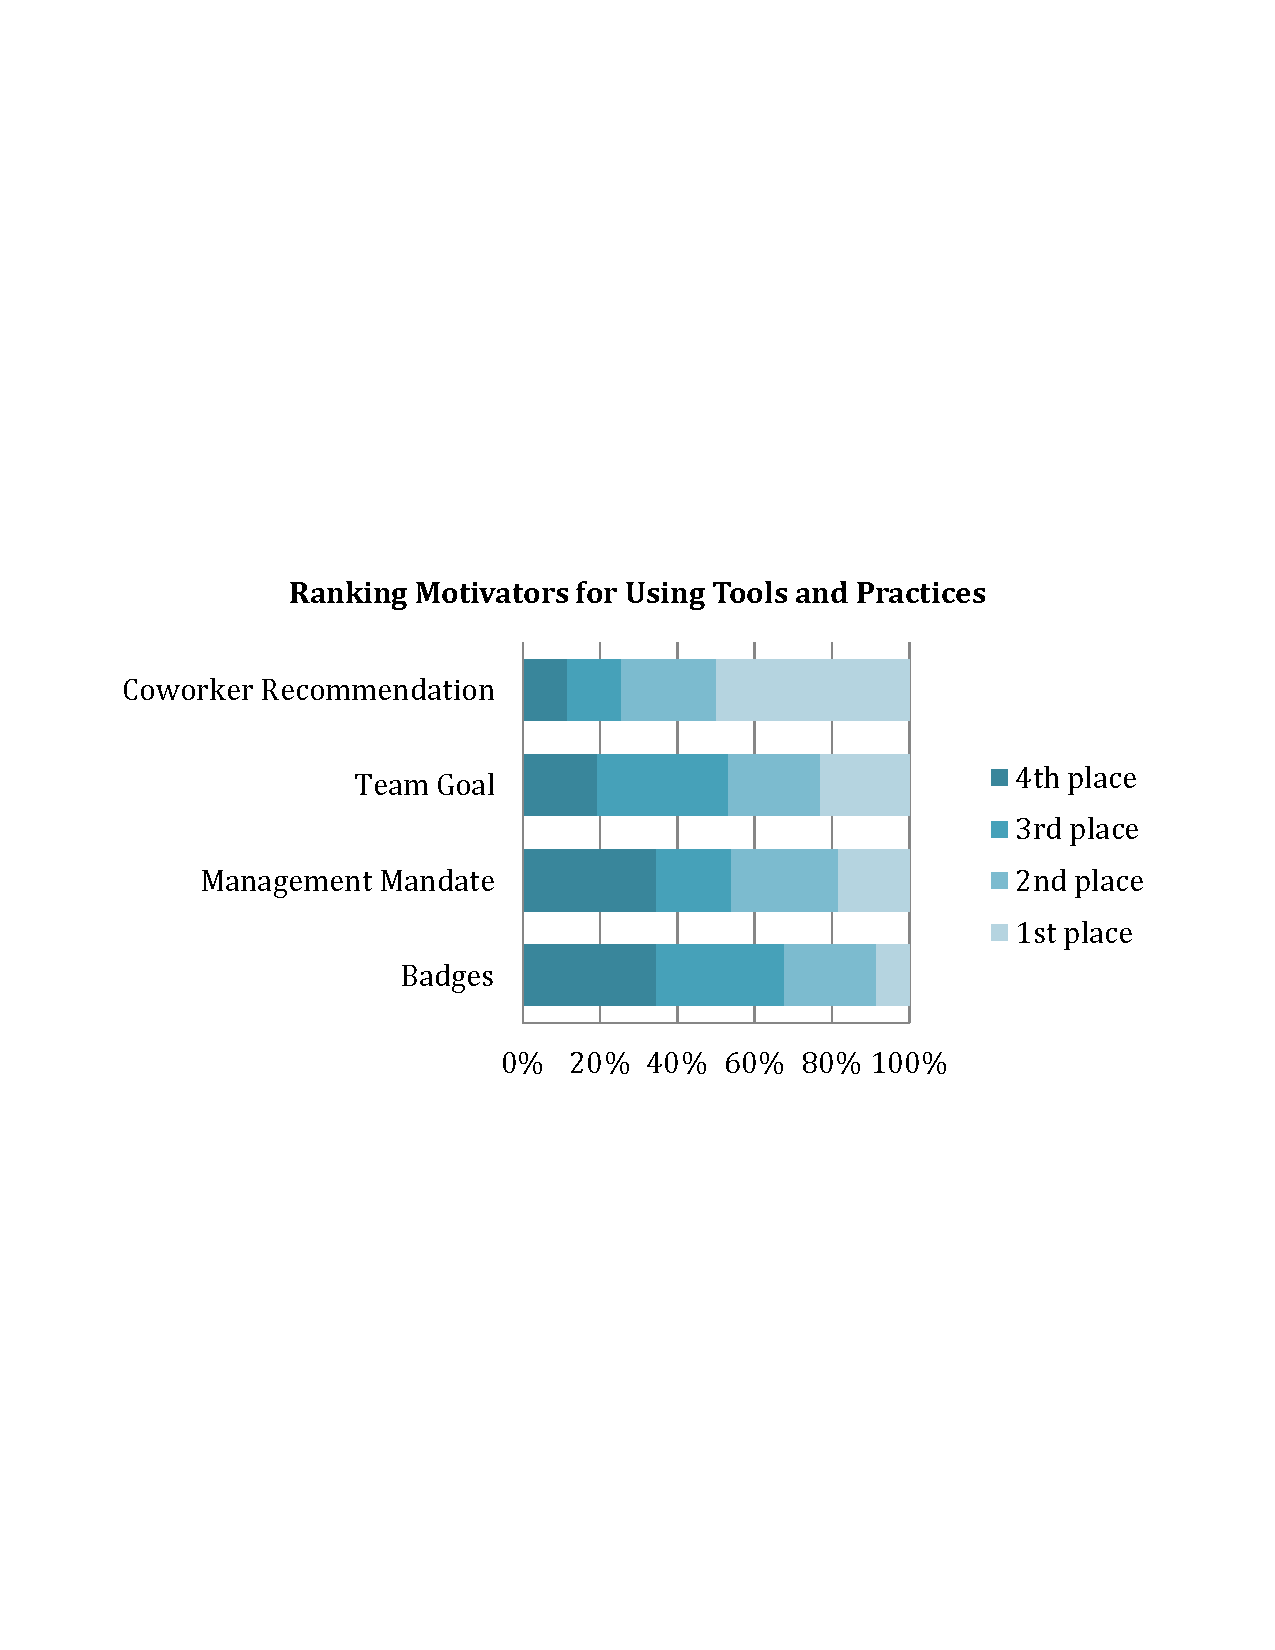
\includegraphics[width=3.4in]{ToolAndPracticeMotivators.pdf}
	\caption{Motivation for using tools and practices}
	\label{fig:toolandpracticemotivators}
\end{figure}

In another question, developers ranked several actions that they would like to receive awards for.  Overall 68\% of developers ranked receiving an award for consistently performing quality practices as either 1st or 2nd place.  Thus, providing awards to developers for using good practices would motivate developers to do them consistently.

 To summarize, the high-level conclusions from each key question are:
\begin{itemize}[itemsep=0mm]
\item 95\% of developers responding would try tools and practices suggested by an automated recommendation system 
\item Developers are motivated by collaboration and team goals more than mandates and individual awards
\item Awards for good quality development practices ranked highest
\item Over 90\% of respondents approved of sharing data with their team members
\end{itemize}
Thus, this pre-study survey provided a positive indicator for going forward with a software engineering tool focused on sharing developer data and rewarding developers for using good practices and tools. 

\section{Game Design}


Following the pre-study findings, we implemented a game-like tool for developers to use in Visual Studio.  The tool focused on motivating the adoption of good practices by including elements of games in the development environment.  The following sections describe how we selected a practice suitable for gamification, designed the game, and included competitive elements in the game.

\subsection{Select a Practice}

We defined the first criteria for selecting a practice based on prior work  applying gamification to other domains outside software development. 
In their paper on game design patterns, Hamari et al. issued a warning that assigning achievements to required tasks reduces intrinsic motivation because player autonomy is reduced by the achievements \cite{wbsnipes:Hamari2011Framework}.  Thus we avoided selecting practices like bug fixing or task completion because they are simply requirements of the job.  

Another criteria imposed by the instrument limits us to practices performed entirely in the IDE so they can be monitored using Blaze.  We identified potential practices of test-driven development, debugging practices, navigation practices,  eliminating static analysis bugs, and frequent CM submissions.  

Frequent CM submission and static analysis bug elimination are highlighted in this paper's related work section with prior gamification studies in classroom environments.  Johnson and Kou achieved automated monitoring of test-driven development practices with Zorro \cite{V:Johnson2007Automated} thus may provide a candidate for future gamification application.   
%reference for debugging?
Debugging practices have developer community opinions on optimal methods, however, detailed debug practices with modern IDEs have not received research community attention, thus are also reserved for future work.  

Studies of developer effectiveness by Robillard et al.\cite{wbsnipes:Robillard2004How} identify structured navigation as a practice more effective developers use when maintaining programs.   Structured navigation fits the requirements of a practice contained in the IDE, has proven benefits, lends itself to measurement and scoring, is not an assigned task, and leaves room for developers to excel.  Thus we selected structured navigation as the practice to demonstrate gamification.

\subsection{Design the Game}

To setup the game, the Blaze tool provides an XML configuration file where the researcher can configure Blaze to categorize and assign points to the commands that are part of a software engineering practice.  Blaze allows the researcher to define multiple command category levels.  Thus we can categorize commands as navigation then further classify them into structured and unstructured navigation.  

We categorize commands as structured navigation when they allow the developer to locate a code element by following the program structure from another element.  These include  built-in Visual Studio commands like Navigate To \textit{Ctrl+,}, Go To Definition \textit{F12}, and Find All References \textit{Ctrl+K,R}  that follow the structured graph of the code.

Commands we considered as unstructured navigation include scrolling through a file using cursor keys or the scroll-bar, opening files from the Solution Explorer, Find commands (e.g. Find in Files), children of these commands (e.g. Find Next), and Go-to line number.

To evaluate developers use of recommended tools in Visual Studio, we categorized them by their tool name.  As part of the pilot, we wanted developers to learn about and adopt the Sando search tool.  Sando is part of the recommended developer tool suite for ABB and supports structured navigation using code search \cite{Shepherd2012Sando}.

Gamification practices consider the feedback of achievements and points as critical to a successful outcome.  The design of achievement awards should gradually encourage the participant to reach higher and higher levels of success in the activity.  Achievements must feel earned to the participant so they recognize the effort to get the award was significant and feel satisfied  \cite{wbsnipes:Hamari2011Framework}.  Hamari and Eranti describe a general relationship between achievements in games and regular game play.     Achievements in games typically create a parallel scoring system to the main game play.  They make the game more engaging by providing multiple ways to increase your score and multiple challenges in one interface.

Considering these guidelines, we assigned one point for each use of structured navigation commands while unstructured navigation commands received zero points.    We gave additional emphasis to using the Sando search tool by assigning ten points for each use.  To create levels following the guidance from Hamari \cite{wbsnipes:Hamari2011Framework}, we applied an exponential curve based on points scored.  Users initially ``level up'' after  working a day or two; the next level may require a week's work to achieve as the difficulty increases.  We designed the points and levels so above average developers can pass all levels during the study period.

By selecting an intact team for the pilot, we hope to leverage aspects of motivation such as the Leaderboard to spur feelings of competition between teammates.    The leaderboard allows developers to see their own score in relation to the top five people on the team.  However, the other participants' identifiers are auto-generated as three capital letters assigned based on their position on the leaderboard.  Not knowing who of your colleagues was ahead of you could reduce motivation, but this avoids one potential source of conflict in an intact team.

\section {Study Design}

Utilizing the continuous monitoring capabilities of Blaze, we designed the pilot to conduct a longitudinal study of the effect of Blaze on developers' navigation practices.  The Blaze tool revealed information about navigation in three stages of one week duration each.  A post-pilot survey gathered developers' opinions of Blaze and some confounding factors that could influence results.

\subsection{Intervention Staging}

Part of the research objective was to determine whether we can drive adoption of a practice through gamification.  As previously discussed, designed the game in Blaze to influence developers towards using more structured navigation practices.  We constructed the interventions during the pilot to roll out in stages each week they use the tool.  This allowed us to establish a baseline and determine the changes as the pilot continued.

In the initial stage, participants were informed of the purpose of the study, and what to expect from the Blaze tool.  The participants installed the tool in their Visual Studio environment.  During this stage, Blaze did not present a window for them to see and simply collected data in the background.   

After a week's data collection marking the end of the first stage, Blaze started to automatically pop-up a window containing a button for a web page with information.  The page included a link to download Sando  and information about using Sando in a video demo.  The sub-page on navigation contained a page of tutorial on the built-in structured navigation commands in Visual Studio.  The ``About Blaze'' page contained details of the point scoring system and background on Blaze's purpose.  The usefulness of the communication site is rated as part of our post-pilot  survey.

In the third stage, developers received instant feedback from Blaze on the points they accumulated during the development session.  The tool's appearance at this stage is shown in Figure \ref{fig:blazeWindow}.  The ``Info'' button provides a level indicator via colored contents and activates a chart display windows when clicked.  Points shows the points accumulated for the developer's history.  Level is the level of the game achieved based on an exponentially growing curve.   The developer could click on the Leaderboard tab to see how their scores compared with the others in the pilot.  This final configuration remained as the display until the end of the pilot.  

\begin{figure}
	\centering
	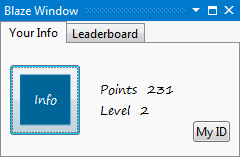
\includegraphics[width=1.6in]{blazeWindow.png}
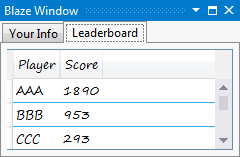
\includegraphics[width=1.6in]{blazeLeaderboard.png}
	\caption{Blaze Tool Window}
	\label{fig:blazeWindow}
\end{figure}


\subsection{Pilot Participants}

As mentioned in Figure \ref{fig:gamification} from our survey, the acceptance of gamification is highest in India. Hence, we conducted this study with an intact team of 6 developers working in an R\&D facility in India on a large industrial software system. Initially, we met the whole team along with the management staff to explain the research project and the Blaze tool we developed. We  explained the aim of the study, what data is collected, and how the data would be processed and managed. 

It was important to gain the confidence of the participants that their data were kept confidential so their activities would be as close as possible to real-world. If the participants felt like they are being tracked and the data would identify them to their peers or managers, then they may refuse to participate or deviate from their normal development style.

We  assured the team about the confidentiality of the data, and the management reassured them that the data collected by the research group will not be used for any other purpose other than the study.  Developers were asked to volunteer for the pilot by their management, however, managers did not know who participated in the study. Their names and data were kept confidential to ensure that no one apart from the research team knows he/she is participating in the pilot.  To distinguish individuals in the data each user is assigned a generated unique ID.  Developers could chose to share the unique ID with us or keep it confidential.  All were willing to share their unique ID with us during the follow-up feedback sessions.   

Management wished to have no knowledge of who was participating and took great care to remain detached from the pilot proceedings.  Data at this level of detail has not been collected in ABB development organizations.  Researchers were careful to create the system where developers controlled whether we could associate their identity with their data, and fortunately management bought into the necessity for participant anonymity.

\subsection{Pilot Survey}

The goal for the pilot follow-up survey was to collect feedback on the tool and the effect it had on the developers' navigation practices and knowledge.  The survey questions were segmented into portions that evaluate prior and post knowledge of navigation practices, key steps in the pilot itself, the influence of game elements on their navigation practices, typical tasks and demographic information.

To find out whether Blaze increased developers'  knowledge of structured navigation commands, we asked them to rate their knowledge of structured navigation commands prior to the pilot on a 1-10 scale.  Then we asked them to contrast their knowledge after the pilot to assess what they learned from the pilot.

The other key question is did Blaze have a perceived effect on their navigation practices.  Here too we asked them to rate how much they used structured navigation prior to the pilot using a 4 choice rating of ``not at all'', ``some'', ``many times'', and ``as much as possible''.  Then we asked whether they used structured navigation commands ``about the same amount'', ``more'',  or ``a lot more'' during the pilot.  These two questions assessed their perceptions of structured navigation command use.  We compared the answers with the usage data collected from Blaze.

The final assessment questions tested whether using Blaze influenced their attention to navigation commands by asking how much specific game elements influenced their practices.  The responses available were ``not at all'', ``a little'', ``some'', and ``a lot''.  

The other questions included whether they reviewed the training materials on structured navigation commands, installed the Sando code search tool, and what types of development tasks they would consider using structured navigation for in general.  Another demographic question asked how well they know the code they work in rated from ``I work in code that I wrote'', ``I maintain code that I am familiar with'', to ``I recently learned the code''.

\section{Results}

\subsection{Pilot Survey Results}

We conducted an in-person post pilot survey in order to cross check the quantitative data from Blaze with developers' perception of their practices and their demographic information.

The pilot survey queried developers' relevant demographic data to help understand some differences in results.  We asked developers to provide their years of experience so we could evaluate any effects experience might have.  The developers in the study had between 7 and 14 years experience.  One developer who dropped out of the study said their lower level of experience compared to their peers influenced their decision to stop participating.  

We asked developers to rate their knowledge of the code they maintain.  Four of the six developers reported they maintain code that they wrote, while the two most experienced developers maintain code that they recently learned.  One developer reported during our individual feedback sessions that working in code they know well affects their navigation practices leading them to use more unstructured navigation.

On the assessment of prior structured navigation knowledge, half of the participants replied they had very good prior knowledge about structured navigation and they use structured navigation ``as much as possible''.  The other half of the participants rated their prior knowledge of structured navigation as good and reported that they use it ``some'' of the time. Of the three developers who rated their prior knowledge and use of structured navigation higher, two of them had the highest point scores of the group.

\begin{figure}
	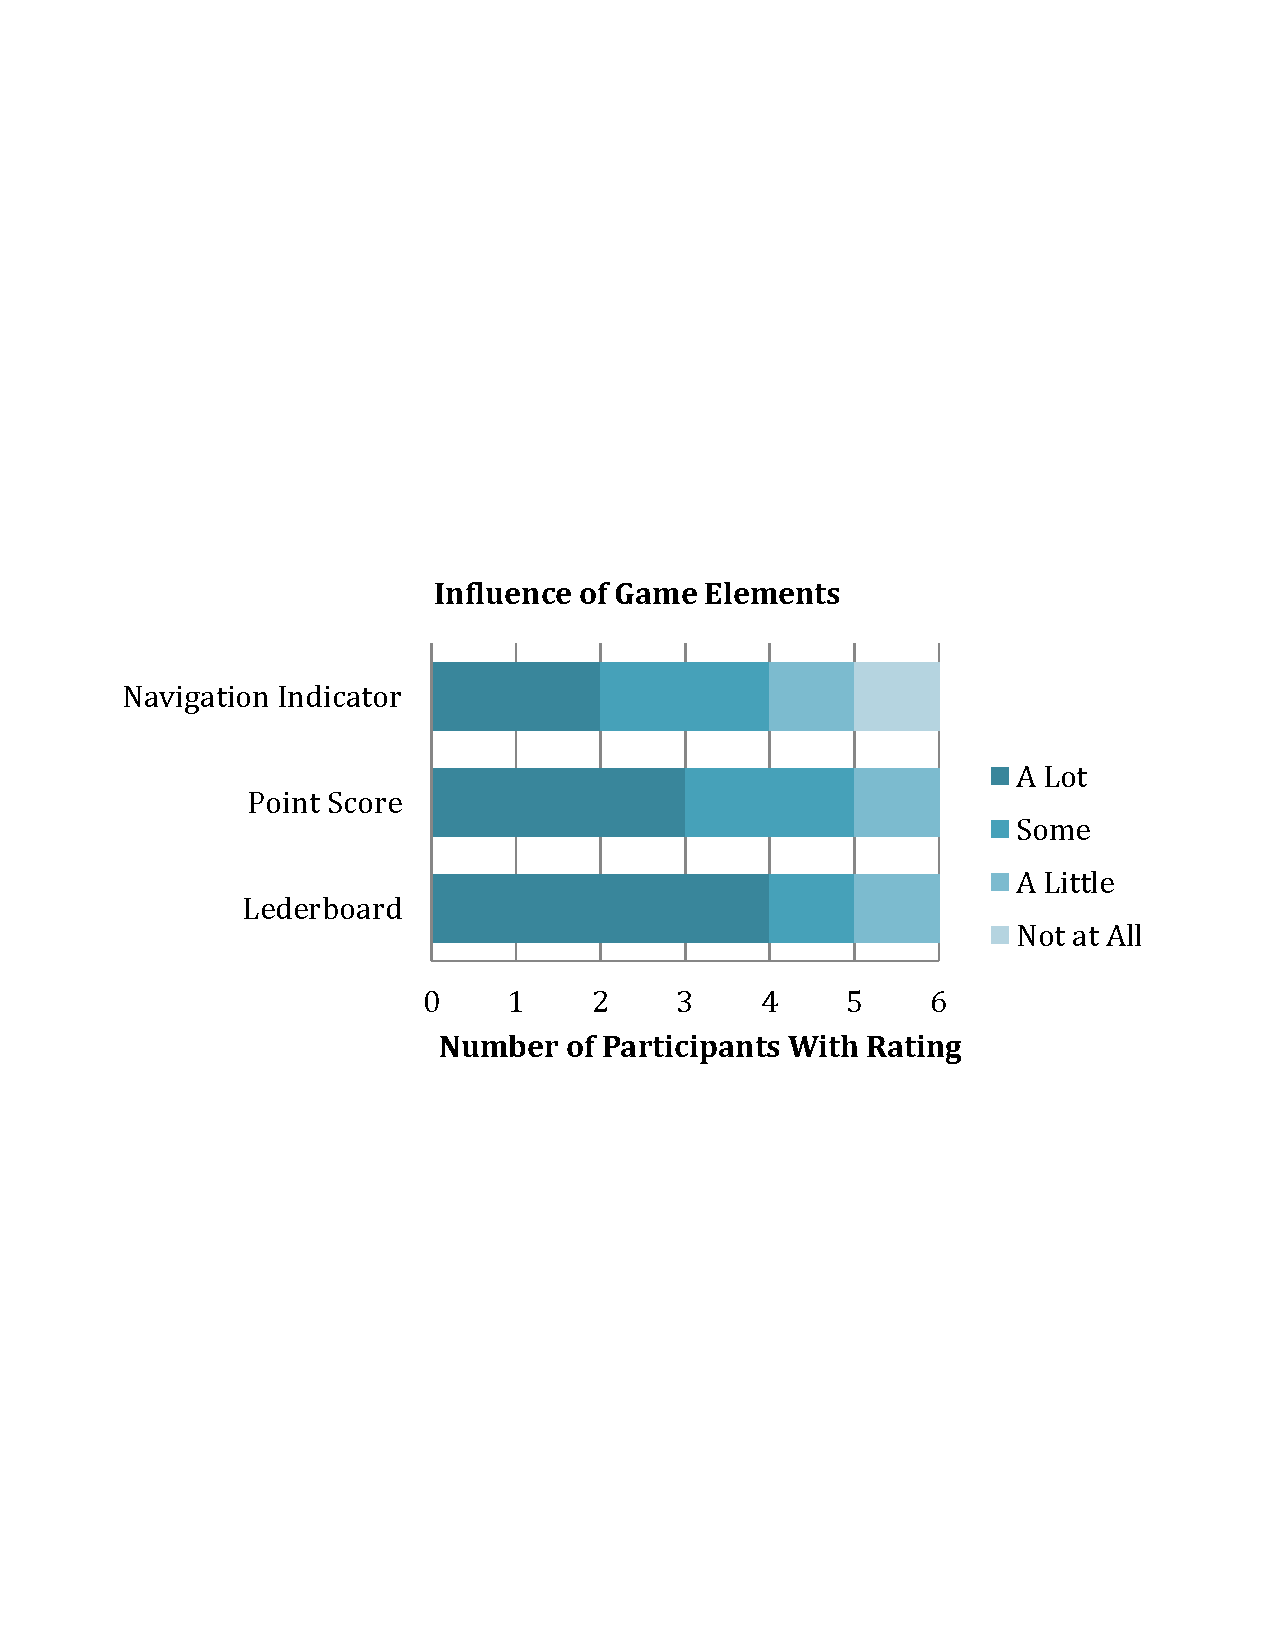
\includegraphics[width=3.4in]{ElementInfluenceChart.pdf}
	\caption{Influence of Feedback Elements}
	\label{fig:elementInfluence}
\end{figure}

The chart in figure \ref{fig:elementInfluence} shows how the individual feedback features influenced developers to think about using structured navigation.  Four out of six developers said the leaderboard influenced them ``a lot'', and all rated the leaderboard as having at least ``a little'' influence.  Three out of six  said their individual point score influenced them ``a lot'', and all said the score had at least ``a little'' influence.  The element with mixed ratings was a graphical indicator on whether they were improving over past use of structured navigation commands.  The indicator received the influencing ``a lot'' rating from two participants and a ``not at all'' influence rating from one participant with the rest having at least ``a little'' influence.  The results indicate the more obvious and more clearly comparative information in the leaderboard was the strongest influence for developers.

The participants requested that Blaze provide more feedback on tips to help them increase their score. They indicated that more obvious feedback, such as hints that pop-up when they launch the tool, would help them more than passively provided information.  Their desire for personal metrics and historical views of the data encourages us that this detailed level of measurement and analysis is perceived as helpful.  Features to meet these requests are part of future work.    

\subsection{Pilot Data Observations}

Blaze logs events from actions the developer takes or actions from Visual Studio itself.  The event is basically a GUI event managed with Visual Studio by event handlers registered with the application to listen for the event.  Blaze becomes a global event handler listening for all events by registering for them in Visual Studio.  

Blaze records key attributes along with each event in visual studio.  The log captures a time-stamp for each event normalized to GMT.  The name of the event provides a low-level classification.  The event type reflects an internal classification in Blaze.  An optional field for Artifact Reference captures data such as the file-name being edited and the currently selected line number.  An anonymized unique identifier for each Blaze user allows us to investigate differences between developers.

To assist in log analysis, Blaze classifies the events into categories for related activities such as navigating, editing, building, debugging,  testing, and using a  known tool.  Each event name maps to a category from the list and sub-division of the navigation category separates structured navigation from unstructured navigation.

In another processing step, Blaze aggregates events along the time-line into sessions.  A session is an abstract concept grouping multiple events into a sequence with a beginning and an end.  Of the many possible ways to define sessions, we chose to define sequences as all the events that transpire before and during a set of edits to a specific file.  When the developer edits a new file, all the events after the last edit to the previous file are included in the new sequence for the new file.  For example, the developer edits file A, then navigates through files B and C finally landing at line 100 of file D where they make another edit.  All the events between the edit of file A and the edit of file D are considered part of the edit session ending with the edit of file D.  Multiple edits to file D that occur before editing a different file are included in the same sequence ending with the edits to file D.  Although not at the method level, this way of generating sequences is similar to how Robillard et al. generated sequences based on located methods for their study \cite{wbsnipes:Robillard2004How}.

\subsubsection{Observations About Drivers of Edit Session Duration}

We selected navigation as the subject of the pilot game because it was identified by Robillard et al.\cite{wbsnipes:Robillard2004How} as correlated with developers who effectively completed a maintenance task.    In this analysis, we ask whether we are focusing on the right area of developers' activity in Visual Studio?

In order to test whether navigation is an important area to address, we construct a hypothesis that using unstructured navigation is an important factor in developer productivity.  Edit session duration, we assert by opinion, is a factor related to developer productivity though there are many other factors we could consider.  With the data available from Blaze, we can explore the categories of events correlated with the duration of edit sessions over the period of the pilot.  

Using Weka\cite{Hall2009WEKA}, we performed an attribute selection process to identify the most significant attributes related to edit session duration.  The attribute search method we chose was Greedy Step-wise search, which selects attributes based on their correlation with the target, and stops adding attributes when the next attribute decreases the correlation.    The top 5 out of the 15 possible categories ranked by this process are as follows:
\begin{enumerate}[itemsep=0mm]
\item Unstructured navigation
\item Debug - events from running the debugger
\item Edit - events that modify the code
\item Other Actions - other events in visual studio that we do not sub-classify
\item Build - events from running a build
\end{enumerate}

To determine the correlation with edit duration, we used R\cite{Rcitation} to construct a linear regression model for unstructured navigation .  The linear model found a positive correlation with unstructured navigation with a p-value <.001 on 1694 degrees of freedom.  The model had an Adjusted R-squared of 0.64 showing a good portion of the variation in edit duration is explained by the unstructured navigation category. 

This analysis shows we cannot disprove that unstructured navigation is correlated with edit duration, thus we conclude it is an important factor in developer productivity.  

\subsubsection{Observations on Navigation Ratio}

To evaluate whether developers improved their practices for structured navigation we established a metric, Navigation ratio, as the number as the number of structured navigation events in a session or period of time over the number of unstructured navigation events.  Our hypothesis is that instant feedback from points combined with game information would result in an increase in the navigation ratio for developers in the pilot.

Structured navigation events included: 
\begin{itemize}[itemsep=0mm]
\item Navigate To (Ctrl+,) is a fuzzy search interface that lists identifiers matching the selected string 
\item Go To Definition (F12) brings up the code that defines the selected identifier 
\item View Call Hierarchy (Ctrl+K Ctrl+T) provides a two way analysis of an identifier's dependencies and uses
\item Class View (Ctrl+W, C) provides a browser and search function for classes and class hierarchy
\item Find All References provides a list of lines that reference an identifier
\item Navigate to Event Handler in the XAML editor shows the event handler for an object
\item View Class Diagram generates a class diagram 
\item View Object Browser is a search tool and browser
\end{itemize}

Unstructured navigation events included selecting a file in an explorer window or selecting the tab for a file, using arrow and page up/down keys to go up/down through a file, scrolling, clicking on a file element, and using any of the built-in find commands such as ``Find in Files'' or ``Quick Find''.

During the pilot, we staged the deployment of information feedback to developers so they would first have access to learn about structured navigation and then get instant feedback in the form of points for using structured navigation commands.  

To evaluate whether developers use more structured navigation when they receive instant feedback, we monitor the change in navigation ratio over the pilot study period.   We expected developers learning about navigation commands and tools that count towards the score would begin using the practices more during the second week.  In the third week, we turn on points feedback and the leaderboard expecting this will encourage developers to use more structured navigation.  

\begin{figure}
	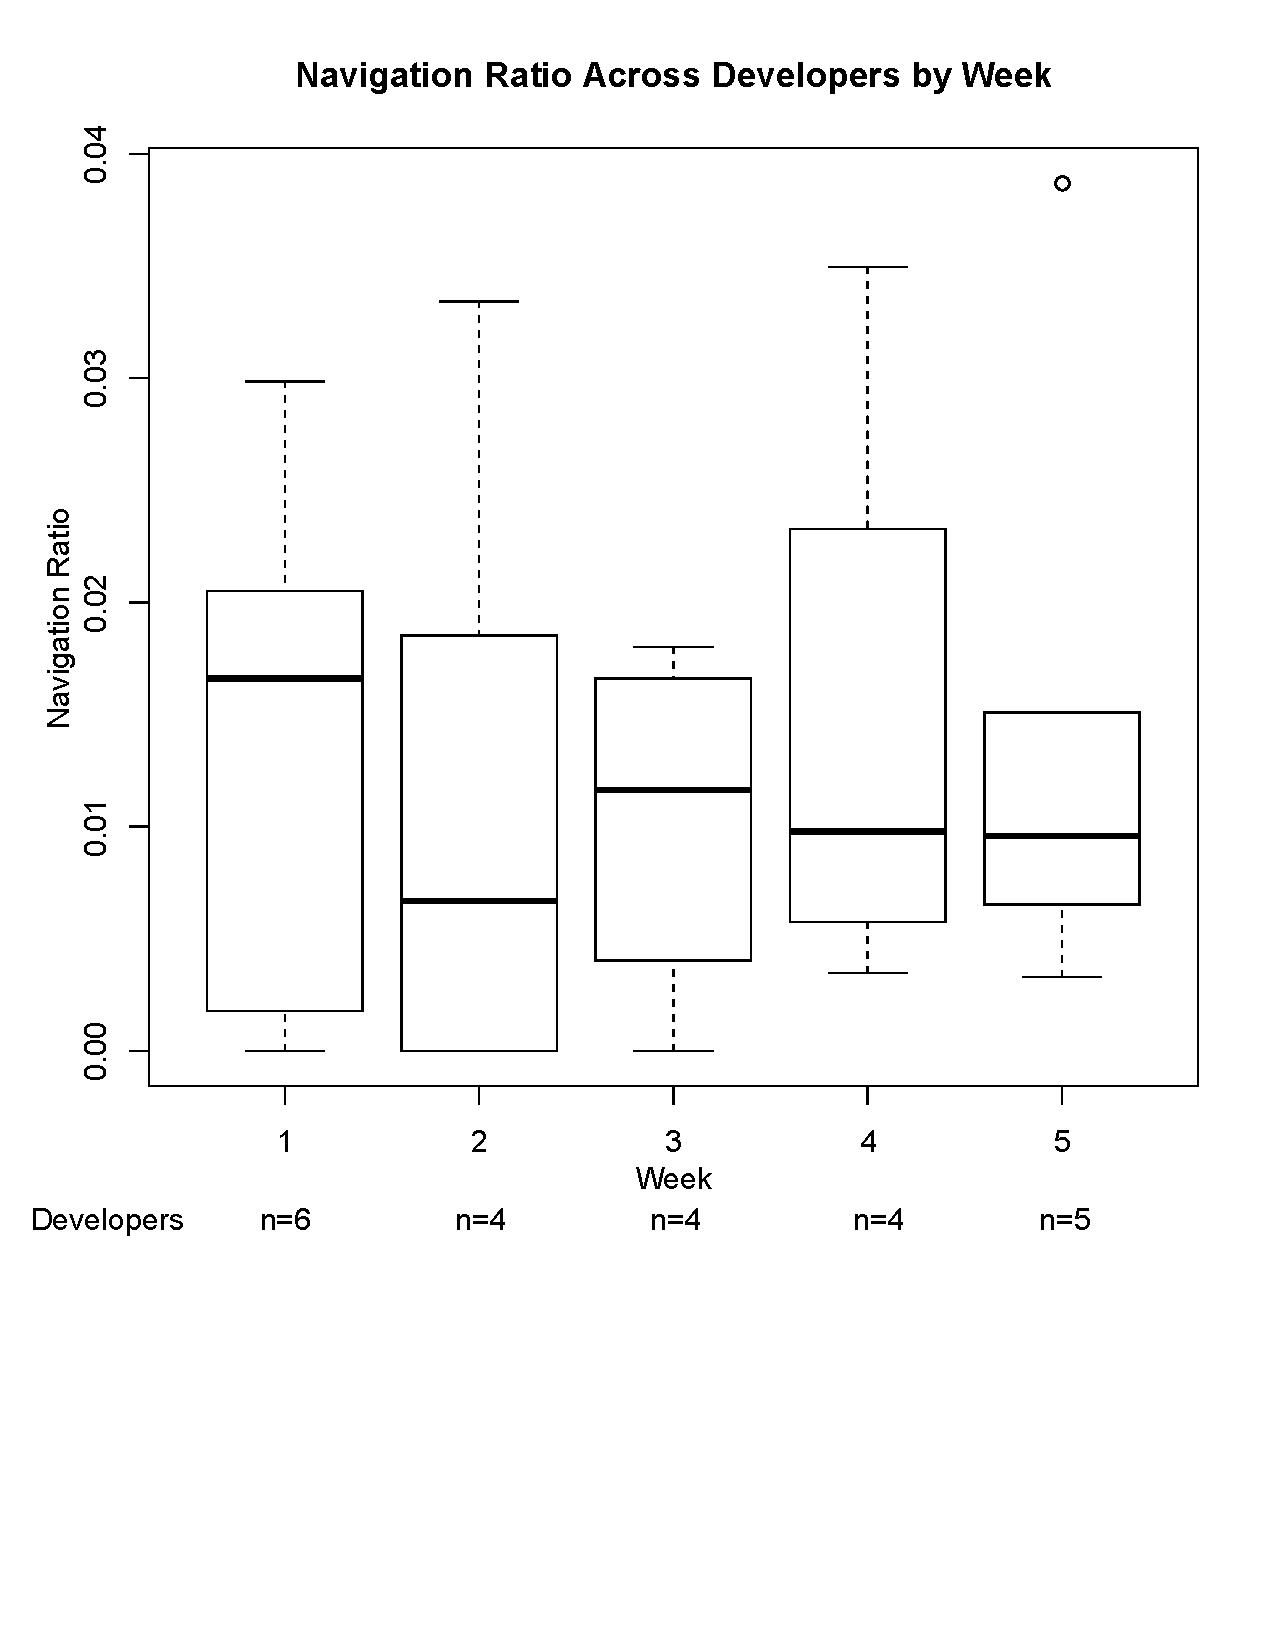
\includegraphics[width=3.3in]{navratioboxplot_ann.pdf}
	\caption{Navigation Ratio by Week}
	\label{fig:navigationaverage}
\end{figure}

We observe visually in Figure \ref{fig:navigationaverage}, that the navigation ratio did not increase significantly from the beginning to the end of the study.  We evaluated the week over week differences using a Wilcoxon Rank sum test \cite{RefWorks:118} comparing week one to week two and week one to week three.    In week two, when the developers were able to learn about structured navigation commands, there was no significant change.  Also in week two, two developers were not providing data.  One was working in another environment and returned to the study, while the other dropped for the rest of the study.  In week three there was a slight increase in the mean, however the increase is not significant.  Weeks four and five follow the formal period of study show the navigation ratio continues in a similar range.  Overall, we did not see a significant effect towards increasing navigation ratio for the interventions Blaze provided to the environment.    

\subsubsection{Observations on Points}

The developers using Blaze received feedback in the form of points given for using structured navigation commands and using the Sando search tool\cite{Shepherd2012Sando}.  Per the pilot design, the points display was disabled until the third week following installation to establish the effect of instant feedback apart from other information.  The points display and the navigation arrow were enabled in the third week to test whether the instant feedback was successful in driving increased use of the targeted features. During the first two weeks shown in Figure \ref{fig:pointsbyweek}, developers were fairly consistent in their use patterns.  With the introduction of the points feedback, two developers' points accumulation spiked in week three due mostly to increased use of Sando.   We informed developers at the beginning of the pilot that Sando usage would receive ten points and using built-in structured navigation commands would receive one point.  

In these results, we see an effect from the points display in Blaze in week three when the developers could see their points feedback for the first time.  We conducted a Wilcoxon Rank sum test on points similar to the way we did for navigation ratio to determine significance.  Across the pilot developers, the difference is not significant at the .05 level. The p-value for week two against week three is .19, and for week one against week three it is .31.  We do know from feedback discussions and usage data that two developers took notice of the points and used Sando more in the third week.  Their use of Sando continued at a lower level in weeks four and five.   The effect of points feedback is greater than navigation ratio during week three because of the additional emphasis of the ten point bonus given for Sando usage.  Results from our post-pilot survey where at least half the developers said the points and leaderboard influenced them "a lot" also supports our conclusion that two developers were influenced by the game elements in Blaze.  

\begin{figure}
	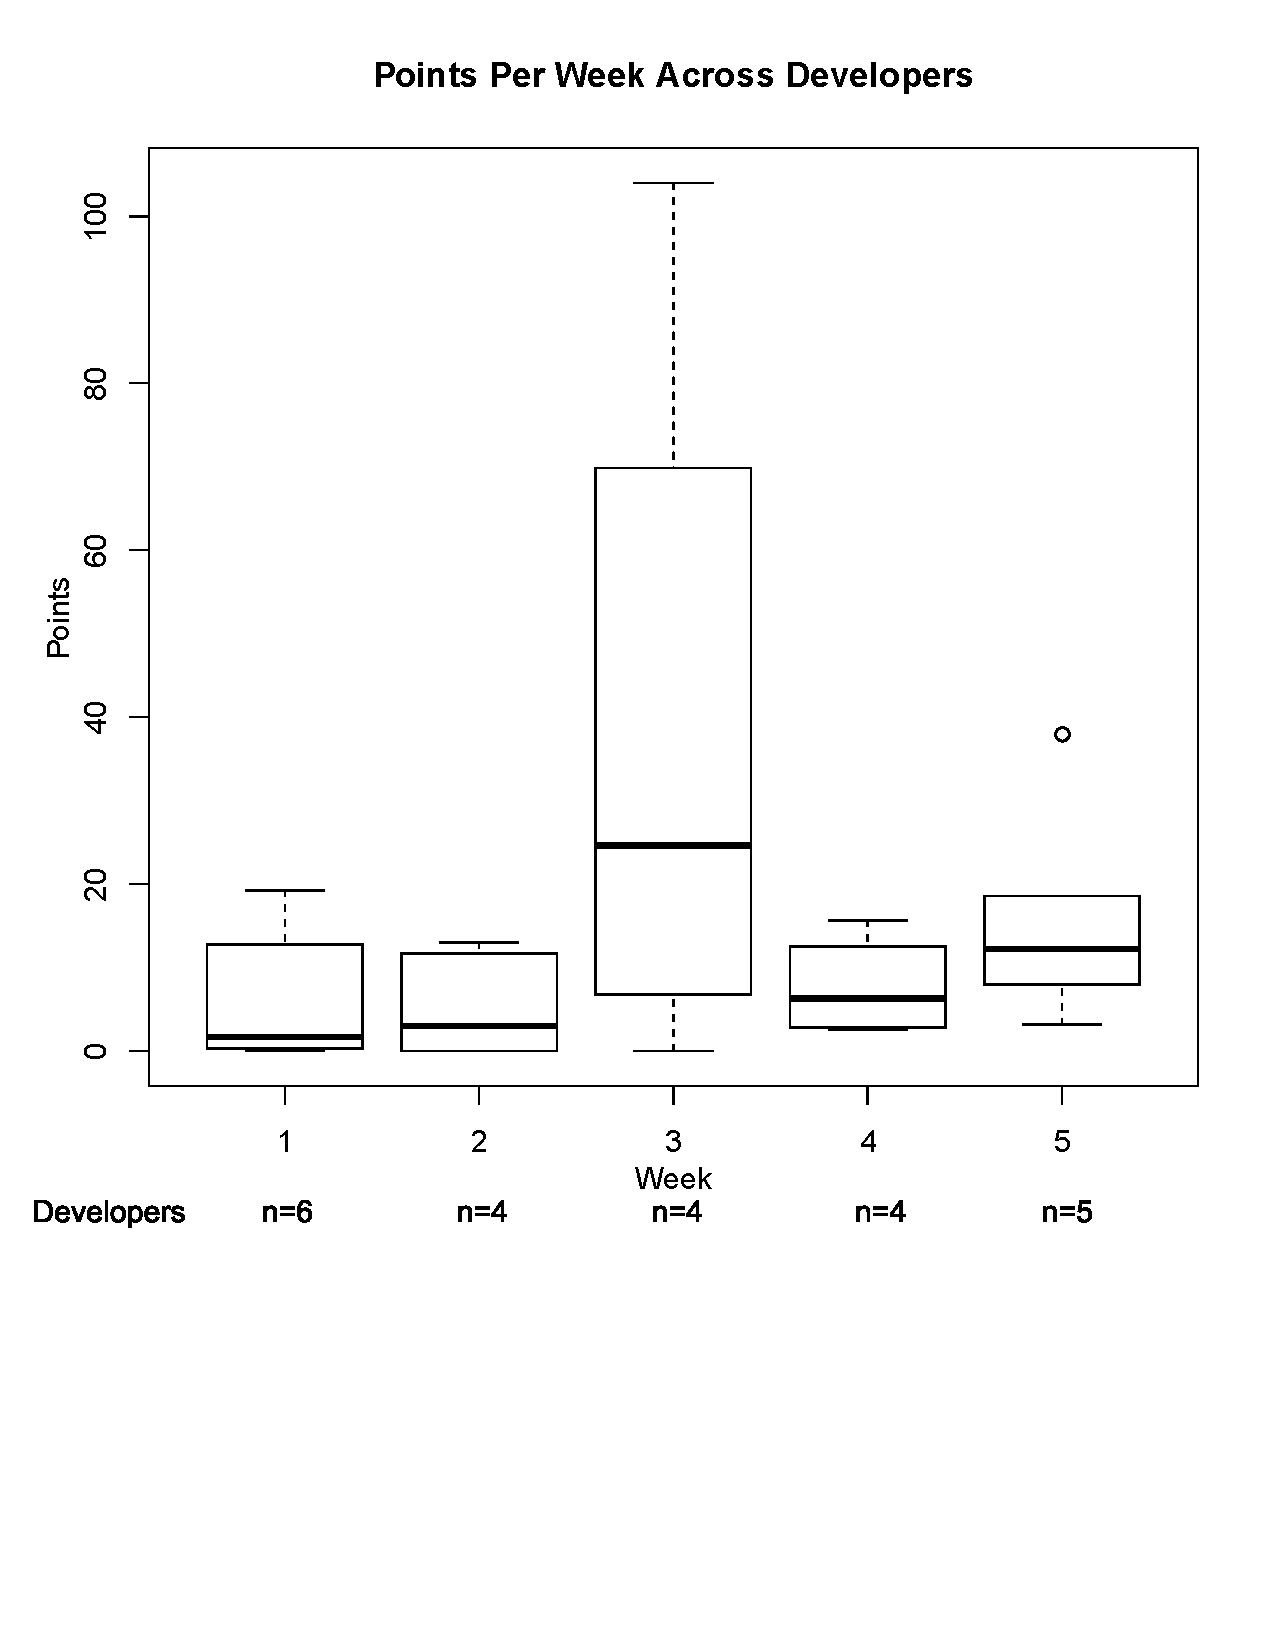
\includegraphics[width=3.3in]{pointsbyweek_ann.pdf}
	\caption{Average Points per Day by Week}
	\label{fig:pointsbyweek}
\end{figure}

\subsubsection{Post-Pilot Feedback Discussions}

Following our data analysis, we conducted one on one feedback sessions with the pilot participants. Before initiating the discussion, we assured the individual developer that the data shared with them is confidential and we will not share the same with management. The participants received the feedback in the form of one-on one presentations of quantitative charts and written analysis of the information.  The key quantitative chart shown in Figure \ref{fig:developercomparison} compared their distribution of time in each category to the median for the group.   

We discovered during these feedback sessions that developers did not spend the entire time in their desktop environment because they had a virtual machine environment available for testing. Thus categories like testing and debugging were affected by whether they used the virtual environment or their desktop for these activities.  Because those categories are not part of navigation, they are not discussed here. The developers use the virtual environment  explains some instances where developers have no activity recorded on some days.  

\begin{figure}
	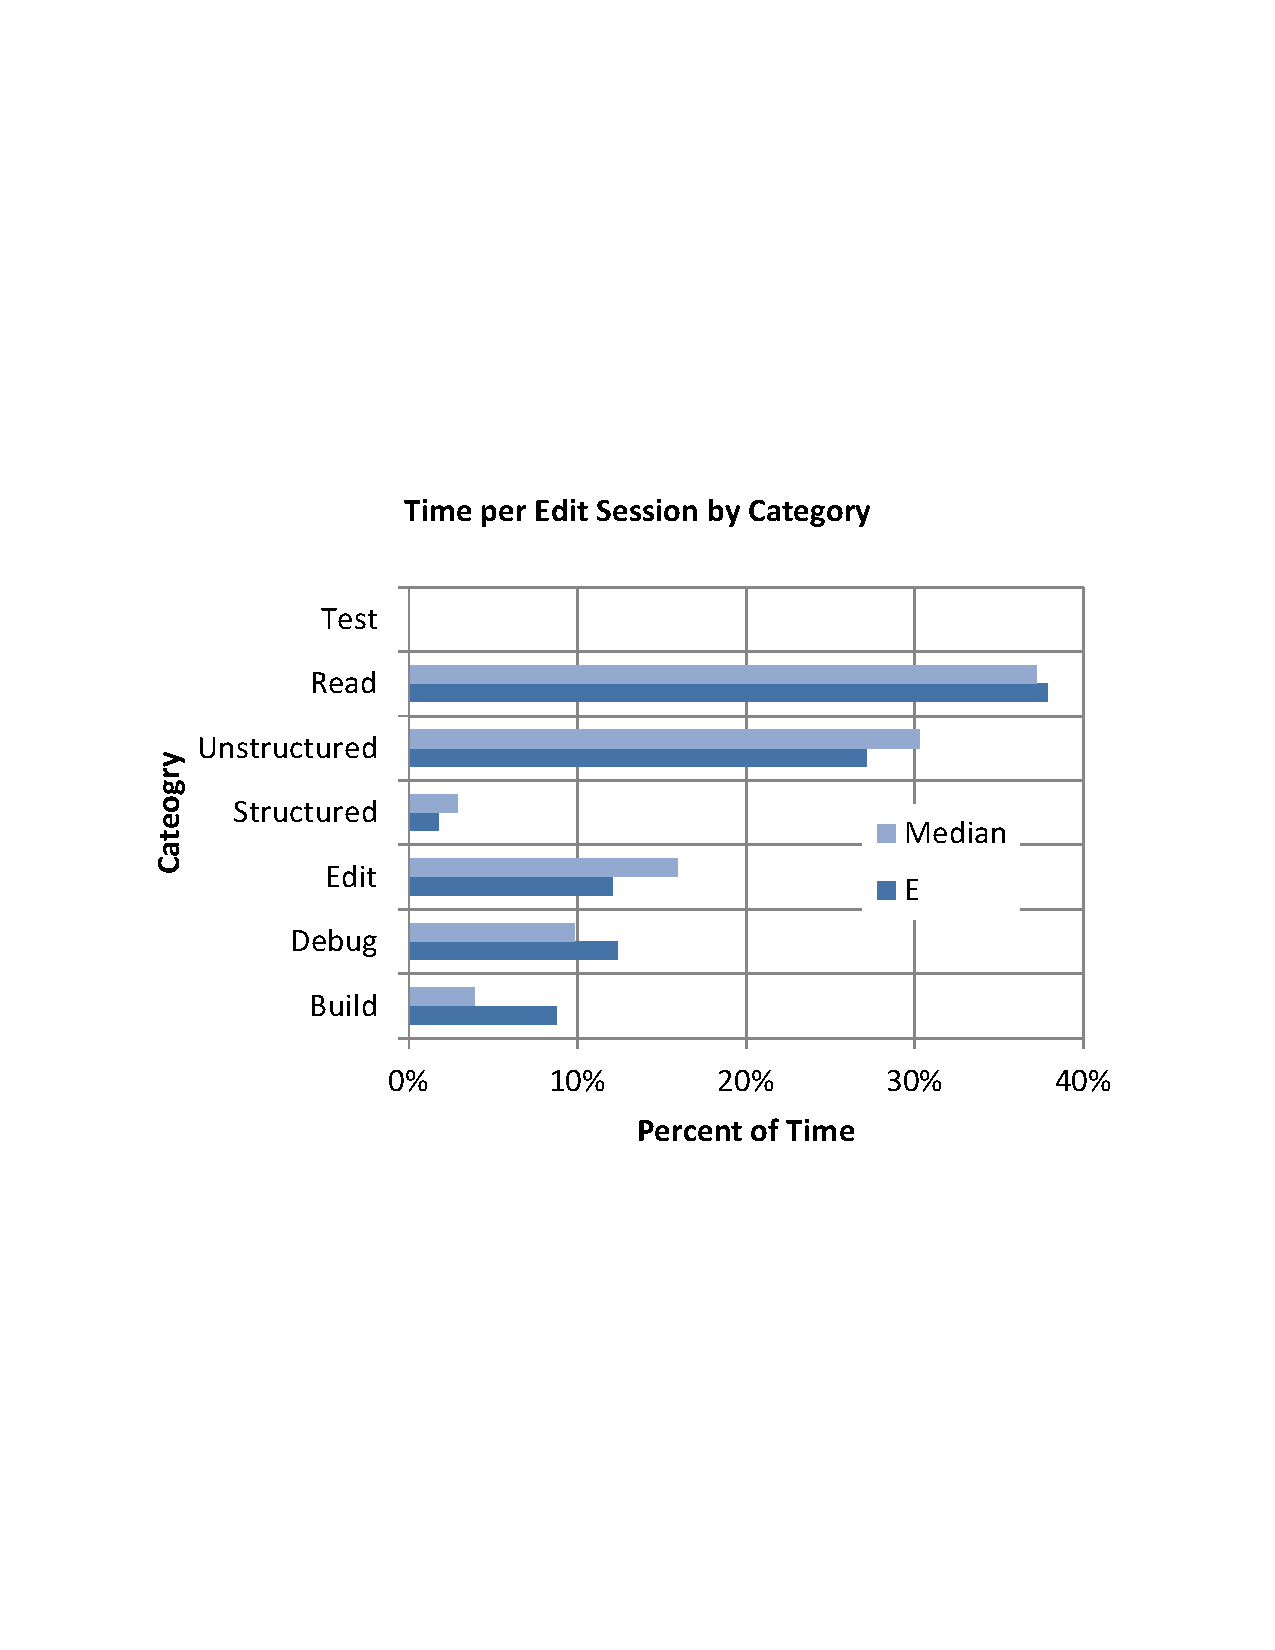
\includegraphics[width=3.3in]{developerEmedian.pdf}
	\caption{Developer Analysis Against Median}
	\label{fig:developercomparison}
\end{figure}


One developer's build effort and the underlying build frequency was much higher than the group median, see Figure \ref{fig:developercomparison}.  We asked the developer to explain how building more frequently helps them. By doing more frequent build, (s)he is trying to ensure the correctness of the work completed so far. The developer feels like (s)he resolves the bugs faster with frequent builds because the code and logic is fresh in her memory. If they build less frequently, even though it reduces the build effort, there are more bugs each time and the developer often spends more time in identifying the problem area than fixing it. Hence the developer feels more frequent builds improves her productivity.  

In another case, we observed a higher level of unstructured navigation than median and asked the developer to explain.  Even though they agree  structured navigation is better than unstructured navigation, (s)he prefers unstructured navigation in some specific instances. The developer is the author of the code and (s)he knows the code completely. ``I know that the line I need to fix is in XYZ method and it is four blocks down from where I am currently. It takes much less time for me to reach the fix location using unstructured navigation. If the code is not written by me, I will prefer structured navigation.'' This instance cautions us to gather information on aspects such as code familiarity and developer experience with the product when assessing the results of a navigation study.

Developers also reiterated how they expected a different experience from Blaze  such as immediate prompts to suggest navigation commands within the context of what they are working on.  This contradicts some developers' comments from the pre-study survey that indicated interruptions from a game would be distracting and unwelcome.

In the feedback, we shared a set of achievement badges tied to specific navigation commands with developers.   Developers said badges would both inform and motivate them to use some specific tools or commands.   This contradicts a result from the pre-study survey where respondents rated badges last in their influence motivating them to improve.  The difference in this opinion may result from the context where developers, when presented with badges, see how badges serve as both a feedback mechanism and guidance on the commands for improving their score and practices.

\section{Threats to Validity}
The threats to construct validity occur when measurements may not reflect the intended operational definition.The key measures of navigation ratio and points in our study could have results differing from their definition.  

Measuring navigation ratio involved categorizing events into structured and unstructured navigation.  The categorization of events is specific to this study and documented herein, however, it may not be accurate to the intent of the operational definition of structured navigation depending on how the developer uses some commands like Find.  Another factor affecting this measurement may occur when developers repeat a command such as hitting the down arrow key many times, that may be something other than navigation (though it is classified as such for this study).  In feedback, we learned developers were reviewing and reading code which may account for these repetitive actions.

The points measurement is more susceptible to influences of simple developer activity compared to navigation ratio.  Thus, a very busy developer could accumulate more points using a lower navigation ratio than a developer who has less activity performed more efficiently.  

Threats to internal validity are those conditions that create alternative reasons for the conclusions, or confound the conclusion.  
The Hawthorne effect, where improvement occurs because we are seeking a change in a particular practice, could impact our results because a presentation  to the pilot organization was required in advance of deployment.  By making the purpose of our measurement and contest known,  we may have triggered the participants to think about navigation commands they use before establishing a baseline.   This threat is mitigated by the data showing four participants did not improve over the course of the study while two demonstrated some improvement.

Participants in the pilot were not randomly selected, they are all volunteers from one intact team chosen due to their advanced practices and understanding of metrics.  Therefore the participants may be predisposed to have an interest in the kind of tool and methodology we are piloting and have bias towards a favorable opinion.  

The intact team may be more familiar with the code they maintain thus be less likely to change their navigation practices.  The post-pilot survey responses confirmed developers are less inclined to use structured navigation when they work in code they are very familiar with.  

Threats to external validity include the fact that the study was conducted in one development location of one company.  Other companies and locations may have different cultures incompatible with this type of monitoring activity.

 Threats to generalizable results exist because we conducted the pilot of the tool with six developers thus the population size is too small to draw statistically significant inferences from. 

 The pilot was conducted in India, the country with the most positive response in our pre-study survey, perhaps where this activity was most acceptable.  Thus, other countries who rated their view of gamification lower may be less receptive. 

Participants in the pilot were professional software engineers with at least seven years of experience.  In other settings where developers have different levels of experience, the results may differ.  In  the pre-study survey, experience was not part of the question set, thus it could have results skewed to a particular age group.

\section{Conclusions}
We set out to demonstrate whether gamification of software development practices could succeed in the industrial environment at ABB.  Through a series of three steps we conducted a pre-study survey with 130 developers, a pilot of a gamified navigation practices with six developers in an intact team using the Blaze tool, and post-pilot survey with the same six developers.  A common thread of findings through all three steps is developers are interested in the idea of using games to help them learn and improve their practices.  On average, 74\% of developers were interested in gamified workspace in our pre-study survey, and five out of six developers indicated elements like points and leaderboards influenced them in our post-pilot survey.  The recorded usage data shows two out of six developers in our pilot responded positively when they started receiving points feedback.  We learned developers need more detailed and immediate feedback from Blaze on ways to improve their practices.  Some developers also appreciated charts providing a historical view of how they spend their time by category compared with the median for the team.  This compliments their feedback on the game showing developers want more information on how to become more effective at their job.  Future work includes providing a mechanism that shares tool recommendations between developers, and allowing developers to share their data with a mentor for feedback.

%ACKNOWLEDGMENTS are optional
\section{Acknowledgments}
The authors wish to thank ABB and the pilot participants in India for their support of this research.

%
% The following two commands are all you need in the
% initial runs of your .tex file to
% produce the bibliography for the citations in your paper.
\bibliographystyle{abbrv}
\balance
\bibliography{mousetap} 
 % sigproc.bib is the name of the Bibliography in this case
% You must have a proper ".bib" file
%  and remember to run:
% latex bibtex latex latex
% to resolve all references
%
% ACM needs 'a single self-contained file'!
%

\end{document}
